% This is samplepaper.tex, a sample chapter demonstrating the
% LLNCS macro package for Springer Computer Science proceedings;
% Version 2.20 of 2017/10/04
%
\documentclass[runningheads]{llncs}
%
\usepackage{graphicx}
\usepackage{tikz}
\usepackage{amssymb}
\usepackage{amsmath}
\usepackage[strings]{underscore}
\usepackage{mathtools}
\usepackage{stmaryrd}

\usepackage{hyperref}
\hypersetup{
	colorlinks=true,
	linkcolor=red,   % internal refs (Definition 3, Figure 1)
	citecolor=red,   % \cite
	urlcolor=blue      % \url / \href
}

\newcommand{\N}{\mathbb{N}}
\newcommand{\Z}{\mathbb{Z}}
\newcommand{\R}{\mathbb{R}}
\newcommand\Slv[2][]{\hspace{-0.9pt}{\curlywedgeuparrow^{#1}}{#2}}
\newcommand\slv[2][]{\hspace{-0.88pt}{\curlywedgedownarrow^{#1}}{#2}}
\newcommand\sqin{\mathrel{\raisebox{0.1ex}{\ooalign{$\sqsubset$\cr $-$}}}}
\makeatletter
\newcommand{\superimpose}[2]{{\ooalign{$#1\@firstoftwo#2$\cr\hfil$#1\@secondoftwo#2$\hfil\cr}}}
\makeatother
\newcommand{\encloses}{\mathrel{\mathpalette\superimpose{{\sqsubset}{\hfil{\raisebox{0.09ex}{\scalebox{0.85}[0.7]{$\sqin$}}}}}}}
\newcommand{\encl}{\mathrel{\raisebox{0.1ex}{$\encloses$}}}
\newcommand{\Str}{\operatorname{Str}}
\newcommand{\supp}{\operatorname{supp}}

\begin{document}

\title{Complex systems as unbounded dynamical holarchies: a framework for understanding emergent phenomena}
\titlerunning{Complex systems as unbounded dynamical holarchies}
\author{Igor Lima Strozzi\orcidID{0000-0003-1792-2880}}
\institute{\textbf{Federal University of Rio de Janeiro}\\
Applied Mathematics Department \\
\url{dma.im.ufrj.br}  \\
\email{istrozzi@matematica.ufrj.br}}
\maketitle

\begin{abstract}
We propose a formal framework for treating complex systems as unbounded dynamical holarchies. The starting point is the simple idea that a system is not merely a set of objects, but a region equipped with parts, relations among parts, and valuations of these relations. From this we define subsystemhood, enclosure, levels and coarse-graining by means of explicit structural transports: data specifying how relational information is inherited, restricted, averaged, rescaled, quotiented, forgotten or generated when one changes scale. A hierarchy is an $\R$-graded coarse-graining flow, and a holarchy is a hierarchy whose interior systems are Janus-faced holons, at once wholes relative to their parts and parts relative to larger wholes. Emergence is localized at coarse-grainings. We prove that systems and structural transports form a category, that the construction conservatively extends restriction-based subsystems, and we carry the framework through a worked example---a glider in Conway's Game of Life---which is structurally but not temporally emergent in isolation and both at a collision. Structurally, it is the failure of a coarse-grained whole to reduce to the non-interacting aggregate of its parts; temporally, it is the failure of a renormalisation-style intertwining between scale and time evolution. A complex system is then an unbounded dynamical holarchy in which both failures persist across a non-trivial band of scales. Scale-invariant, or self-similar, holarchies and their simulation are left to future work.
\keywords{Complex systems \and Holarchy \and Emergence \and Multilevel systems \and Coarse-graining.}
\end{abstract}

\section{Introduction}

As our knowledge about a phenomenon increases, what once appeared simple often becomes complicated again. The gain is not only the addition of more facts. It is also a change in the way the object is cut: new parts appear, old boundaries become questionable, and relations that were invisible at a previous resolution begin to matter. In this sense, complexity is not merely a matter of having many components. It is also a matter of not knowing, in advance, which components and which scale of description are the adequate ones.

A gas may be described by molecules, by regions carrying temperature and pressure, or by macroscopic flows. A cell may be an object in a tissue, a system of organelles, or a physical region filled with molecular interactions. None of these descriptions is simply false. Each is a cut through a larger structure of possible descriptions, and the usefulness of each cut depends on the question one wants to answer. The difficulty is that the cuts do not live independently from one another. The temperature of a region is not foreign to molecular velocities; tissue behaviour is not foreign to intracellular processes; and yet the coarser description is not, in practice or in concept, a mere copy of the finer one.

This suggests that complexity is not well captured by a single state space at a single level. Classical dynamical systems theory is indispensable, but its usual form presupposes what many complex systems tend to destabilize: fixed variables, fixed boundaries and a privileged scale of description. In complex systems the state space may expand, contract or change type; the boundary between system and environment may depend on the question; and the behaviour observed at one level may be produced only by changing what counts as an element at another. The problem is therefore not only to describe a dynamics, but also to describe how the object of the dynamics changes when the level of description changes.

The present paper develops a compact formal language for this situation. We take a system to be a set-theoretic region equipped with elements, relations and valuations of relations. The non-standard choice is that elements are not points of the underlying set, but disjoint parts of it. This makes the framework naturally mereological: a system can be refined by subdividing its elements, or coarsened by aggregating them, without leaving the same category of objects. The resulting formalism is intentionally close to spatial intuition, but it is not meant to be restricted to metric spaces. Rather, the spatial picture is used as a guide for keeping boundary, inclusion and resolution in the same language.

The central mechanism is \emph{structural transport}. When one passes from one level to another, relational data do not merely reappear unchanged. They may be inherited, averaged, quotiented, projected, rescaled, forgotten or newly generated from several lower-level data at once. For instance, the temperature of a region is not one molecular velocity; it is a transported macroscopic quantity obtained from many microscopic degrees of freedom. Similarly, the behaviour of a cell in a tissue is not just a relabelling of its molecules, since the relevant relations at the cellular level depend on a different organization of parts and context. The point of naming this transport is to avoid hiding the modelling step precisely where emergence is usually invoked.

Emergence is then treated locally. Instead of saying that a whole is emergent in some global and obscure sense, we ask whether the coarse-graining that produces the whole is reducible to the non-interacting aggregate of its parts. If it is not -- because it introduces contextual extent or inter-part coupling -- the whole is structurally emergent. We also ask whether time evolution commutes with coarse-graining, up to a scale-dependent time rescaling. Its failure gives temporal emergence. Thus the intuitive idea that a whole is more than the sum of its parts is translated into a question about the maps that carry structure and dynamics across scales.

The holarchic view enters at this point. The same entity can be a whole at one level, a part at another, and a dynamical unit across time. A cell is made of subcellular parts and at the same time is a part of a tissue; an organism is a whole relative to organs and a part relative to an ecosystem; even in artificial life, a coherent particle cluster may be a whole relative to its particles and a part of a larger aggregate. To model this without privileging one level, we shall treat complex systems as unbounded dynamical holarchies.

The original motivation was the study of self-similar nested systems: holarchies in which the transition between consecutive levels preserves enough form to deserve being called scale-invariant. That problem requires a similarity theory for systems and transports, and is postponed. The present goal is more basic: to define systems, structural transports, coarse-grainings, holons, holarchies and the two corresponding notions of emergence, in a way that is formal enough to support later simulation but still close to the conceptual pressure that motivates it.

The exposition therefore alternates between two registers. On the one hand, we give definitions, since without them the discussion of emergence tends to remain metaphorical. On the other hand, we keep the motivating examples close, because the definitions are not meant to replace the intuition but to discipline it. A complex system is not made clearer by being forced too early into a rigid formal skeleton. It is made clearer when the skeleton records the modelling decisions one was already making: where the boundary is drawn, what the elements are, which relations are retained, and how a coarser description is obtained from a finer one.

\paragraph{Relation to existing accounts.}
The framework complements rather than replaces several existing approaches. Weak emergence in the sense of Bedau \cite{Bedau1997} marks macro-facts derivable from micro-dynamics only by simulation; our temporal defect (Definition~\ref{def::dyn}) is a structural counterpart that locates this irreducibility in the failure of the scale--time intertwining. Causal emergence \cite{Klein2020} measures, information-theoretically, when a coarse description carries more effective information than its substrate, but works over a fixed state space, whereas here parts, boundary and state space may themselves change with scale. Computational mechanics \cite{Crutchfield1994} builds the minimal predictive model of a process, and its statistical complexity is a provenance measure to which our essential-support condition (Definition~\ref{def::emerg}) is a mereological analogue. Rosen's $(M,R)$ systems \cite{Rosen1991} demand organisational closure; our holons are whole/part but not assumed closed. Operadic, wiring-diagram accounts \cite{Spivak2013} compose fixed-interface boxes, whereas our category of transports (Proposition~\ref{prop::cat}) lets the very inventory of relations be transported across scales. The renormalisation group \cite{Wilson1975,Kadanoff1966} is the canonical scale flow whose intertwining Definition~\ref{def::dyn} borrows, and the hierarchy-theoretic tradition \cite{Simon2012,Salthe1985,Wimsatt1994} supplies near-decomposability and levels, which the $\R$-graded flow makes continuous. What the holarchic framework adds over each is a single object in which parts, levels, boundary change, structural emergence and temporal emergence are separately definable and separately checkable.

\section{Background and scope}

We use systems theory in a broad sense, drawing on general systems theory, dynamical systems theory, multi-level systems, holonic multi-agent systems and nested systems. General systems theory supplies the guiding intuition of interrelated elements, but usually leaves the boundary problem underdetermined: it is not always clear where the system stops and its environment begins. Dynamical systems theory supplies time evolution, but typically fixes the state space and therefore has difficulty with systems in which elements appear, disappear or change type. Multi-strata systems describe several levels, but often make the passage between levels too restrictive. Holonic multi-agent systems formalize whole--part agents, but are tied to agency and coordination. Nested-system approaches emphasize enclosure, sometimes at the cost of building emergence into nestedness itself \cite{Backlund2000,Mesarovic1970,Mesarovic1976,Fischer2003,Koestler1967,Walloth2016}.

The framework below keeps these ingredients separate. A system may be nested without being emergent; a hierarchy may have many levels without being holarchic; a holarchy may be static before being equipped with dynamics. This separation is not merely pedantic. If emergence is placed directly in the definition of nestedness or complexity, then one cannot ask whether a given passage between levels is emergent. One has already answered by terminology. Here, instead, emergence is a property of a specified coarse-graining, and this makes the concept both more modest and more useful.

Our intended examples are spatial or spatially interpretable. The underlying set can be read as a region, the elements as subregions, and the scale parameter as resolution. Particle life, cellular automata and Lenia are natural test cases \cite{Gardner1970,Chan2019}: they make visible how coherent objects appear from simple rules, persist for some time, merge, split or disappear. A glider in a cellular automaton is not one cell; it is a pattern across cells. A particle-life ``organism'' is not a single particle; it is a moving aggregate with internal organization. The present paper does not simulate these systems. It gives a formal domain in which such simulations could later be analysed without having to decide, beforehand and once for all, which level is the true one.

\section{Systems and structural transport}

We fix a few conventions. If $S$ is a set whose elements are sets, $\bigcup S=\{e\mid e\in x\text{ for some }x\in S\}$. We write $\N_{\leq n}=\{0,1,\ldots,n\}$, $\Z^+=\{1,2,\ldots\}$ and $\Z^- =\{-1,-2,\ldots\}$. A family $\{S_i\}_{i\in I}$ may be denoted simply by $\{S_i\}$ when the index set is clear. We use standard first-order structures in the background sense of \cite{Poizat2000}, but separate the incidence of a relation from the value it carries.

\begin{definition}[Valued relation]\label{def::vrel}
Let $I$ be finite, $|I|=n$, let $S=\{S_i\}_{i\in I}$ be a family of sets, and let $R\subseteq \prod_{i\in I}S_i$ be an $n$-ary relation. A $v$-valued relation over $S$ is a triple
\[
R_v=(R,V,v),\qquad v:R\to V,
\]
where $V$ is a set of values. We write $v(R)=\{v(r)\in V\mid r\in R\}$ and call $R$ the underlying relation.
\end{definition}

Thus a valued relation is an $(n+1)$-ary relation functional in its value coordinate. The point is not logical novelty, but bookkeeping. The underlying relation records which tuples interact; the valuation records how they interact, for instance by weights, intensities, probabilities, distances or qualitative labels. This distinction will be useful later because a change of level may preserve incidence while changing values, or preserve a value-like quantity while altering the relation on which it is defined. A graph quotient, for example, may keep track of which coarse blocks interact but replace many edge weights by a single aggregate weight.

\begin{definition}[System]\label{sys}
Let $S$ be a set, $|S|\geq 2$, let $\mathfrak P$ be a partition of $S$, and let $\Gamma_{\mathfrak P}\subseteq\mathfrak P$ have cardinality $C$. For each $k\in\N_{\leq C}$ let $R_k=\{R_{ki}\subseteq \Gamma_{\mathfrak P}^{k}\mid i\in\N_{\leq n_k}\}$ be a family of $k$-ary relations over $\Gamma_{\mathfrak P}$. For each $R_{ki}$ let $P_{ki}$ be a possibly empty set of valuations (Definition~\ref{def::vrel}) $v_{kij}:R_{ki}\to V_{kij}$. Put
\[
\mathbf R=\{R_k\mid k\in\N_{\leq C}\},\qquad
\mathbf V=\{P_{ki}\mid k\in\N_{\leq C},\ i\in\N_{\leq n_k}\}.
\]
A system is a quadruple
\[
\mathcal S=(S,\Gamma_{\mathfrak P},\mathbf R,\mathbf V).
\]
We write $\mathfrak u(\mathcal S)=S$, $\mathfrak e(\mathcal S)=\Gamma_{\mathfrak P}$, $\mathfrak r(\mathcal S)=\mathbf R$ and $\mathfrak v(\mathcal S)=\mathbf V$. A non-empty $s\subseteq S$ is an element of $\mathcal S$, written $s\sqin\mathcal S$, iff $s\in\Gamma_{\mathfrak P}$. For a system $\mathcal S'$, we extend this by $\mathcal S'\sqin\mathcal S$ iff $\mathfrak u(\mathcal S')\in\mathfrak e(\mathcal S)$.
\end{definition}

Properties are unary relations with valuations; constants may be treated as $0$-ary operations or parameters. The unusual feature is that elements are disjoint subsets of the underlying set rather than points. This is what allows the same object to be an element of a larger system and, if resolved further, a system in its own right. Under the spatial reading, the underlying set is the region in which the system is found, whereas the elements are the pieces of that region recognized by the description. If the description changes, the region may remain comparable while the pieces change. This is the reason for building the mereological aspect into the definition rather than adding it afterwards.

For a system $\mathcal S$, set
\[
\Str_r(\mathcal S)=\bigcup\mathfrak r(\mathcal S),\qquad
\Str_v(\mathcal S)=\bigcup\mathfrak v(\mathcal S),\qquad
\Str(\mathcal S)=\Str_r(\mathcal S)\sqcup\Str_v(\mathcal S),
\]
where the coproduct tags each datum as relational or valuational. A datum of sort $v$ is a whole valuation function, not an isolated value.

\begin{definition}[Structural transport]\label{def::transport}
Fix a class $\mathfrak F$ of admissible operations: partial functions on finite tuples of structural data, closed under composition and finite products and containing all coordinate projections. Let $\mathcal A$ and $\mathcal B$ be systems. A structural transport from $\mathcal A$ to $\mathcal B$, written
\[
\Theta:\mathcal A\rightsquigarrow\mathcal B,
\]
assigns to each $Q\in\Str(\mathcal B)$ a tuple $\sigma_Q\in\Str(\mathcal A)^{p_Q}$ and a map $F_Q\in\mathfrak F$, sort-compatible, such that
\[
Q=F_Q(\sigma_Q).
\]
The \emph{(essential) support} $\supp_\Theta(Q)\subseteq\Str(\mathcal A)$ is the set of entries $\sigma_{Q,j}$ on which $F_Q$ genuinely depends, i.e.\ in which it is non-constant; a constant map has empty support and a coordinate projection a singleton one.
\end{definition}

\noindent\emph{Convention (a canonical $\mathfrak F$).} Unless stated otherwise, $\mathfrak F$ is the smallest class closed under composition and finite products that contains the coordinate projections and relational restrictions (on sort-$r$ data), the finite weighted sums and averages of real-valued valuations (on sort-$v$ data), and the quotient maps induced by equivalence relations on $\Gamma_{\mathfrak P}$. This expresses the coarse quantities used below---centroids, block-averages, restrictions, quotients---while excluding the constant maps that would make every coarse datum vacuously transportable.

The definition is deliberately data-sensitive. If one merely asked that $Q$ be obtainable from $\Str(\mathcal A)$, constant maps would trivialize the notion. A transport records how $Q$ is obtained. In a gas, a macroscopic pressure relation may be transported from many molecular momenta; in a graph model, a coarse edge weight may be transported from a cut, a quotient or an average of fine edges; in an artificial-life model, the velocity or orientation of a coherent aggregate may be transported from the positions and velocities of many particles. The important point is that these are not the same modelling operation, even if all of them are informally called ``coarse-graining''.

This is also where the framework tries to remain close to computation. In an implementation, one must actually store or compute the passage from fine data to coarse data. One chooses a quotient, an average, a threshold, a clustering rule, a projection, or something more elaborate. The structural transport is the formal counterpart of this choice. Transports compose in the evident way, giving the following.

\begin{proposition}[The category of transports]\label{prop::cat}
Fix $\mathfrak F$. Systems and structural transports form a category $\mathbf{Sys}_{\mathfrak F}$, in which $\mathrm{id}_{\mathcal A}$ assigns to each $Q\in\Str(\mathcal A)$ the pair $((Q),\mathrm{pr}_1)$, and the composite of $\Theta:\mathcal A\rightsquigarrow\mathcal B$ and $\Psi:\mathcal B\rightsquigarrow\mathcal C$ assigns to $Q\in\Str(\mathcal C)$, with $\Psi$-datum $(\boldsymbol\tau_Q,G_Q)$ and $\boldsymbol\tau_Q=(B_1,\dots,B_k)$, the concatenated tuple $\sigma_{B_1}\frown\cdots\frown\sigma_{B_k}$ and the map $G_Q\circ(F_{B_1}\times\cdots\times F_{B_k})$. Two transports are identified when, for every $Q$, they have the same essential support and induce the same map on it---equivalently, the same $(\sigma_Q,F_Q)$ up to a permutation of slots in which $F_Q$ is symmetric; this identification is a congruence for composition, so $\mathbf{Sys}_{\mathfrak F}$ is well defined.
\end{proposition}
\begin{proof}
The composite map lies in $\mathfrak F$ since $\mathfrak F$ is closed under composition and finite products, and is sort-compatible since each factor is. Composition is associative because finite tuples form the free monoid under concatenation, so $(\sigma\frown\sigma')\frown\sigma''=\sigma\frown(\sigma'\frown\sigma'')$ and the corresponding product maps coincide. The projection identities are two-sided units: composing with $\mathrm{id}$ replaces each $B_j$ by $(B_j)$ under $\mathrm{pr}_1$, leaving $\sigma_{B_j}$ and $F_{B_j}$ unchanged. Finally the identification is a congruence: if $\Theta_1\sim\Theta_2$ and $\Psi_1\sim\Psi_2$, then $\Psi_1\circ\Theta_1\sim\Psi_2\circ\Theta_2$, since the essential support of the composite at $Q$ is the union of the factors' essential supports over the $B_j$ in $\supp(G_Q)$, and the induced map on it is $G_Q\circ\prod_j F_{B_j}$ up to permutation of symmetric slots---both fixed by the factors' equivalence classes alone.
\end{proof}

There is a small but important asymmetry here. A transport from fine to coarse data may be many-to-one and may deliberately lose information. This is not a defect. It is often exactly what a model is supposed to do. What matters is that the loss, aggregation or transformation is explicitly carried by the transport rather than left in the informal phrase ``passing to the macro level''. Later, when we ask whether a whole is reducible to its parts, we will be asking a question about this specified transport, not about an unspecified philosophical relation between wholes and parts.

\section{Subsystems, levels and coarse-graining}

The usual idea that a subsystem is obtained by restriction is too narrow for the present aim. A subsystem may inherit relations, but it may also carry rescaled or context-dependent relations. Conversely, a superlevel may not preserve all lower-level data: it may discard micro-detail and retain only variables relevant to a coarser description. This is already visible in ordinary modelling. A region of a gas is a subsystem of the container, but the variables one assigns to it may depend on measurements or averages involving the whole gas. A cell is a subsystem of a tissue, but its effective behaviour may depend on surrounding cells and extracellular context.

\begin{definition}[Subsystem]\label{def::subsyst}
A system $\mathcal S'=(S',\Gamma'_{\mathfrak P'},\mathbf R',\mathbf V')$ is a weak subsystem of $\mathcal S=(S,\Gamma_{\mathfrak P},\mathbf R,\mathbf V)$ (Definition~\ref{sys}), written $\mathcal S'\sqsubseteq\mathcal S$, if $S'\subseteq S$, $\bigcup\Gamma'_{\mathfrak P'}\subseteq\bigcup\Gamma_{\mathfrak P}$, and there is a structural transport (Definition~\ref{def::transport})
\[
\Theta:\mathcal S\rightsquigarrow\mathcal S'
\]
producing every relation and valuation of $\mathcal S'$. It is a proper subsystem, written $\mathcal S'\sqsubset\mathcal S$, when moreover $\mathfrak u(\mathcal S')\subsetneq\mathfrak u(\mathcal S)$.
\end{definition}

Weak subsystemhood is reflexive and transitive by identity and composition of transports; proper subsystemhood is a strict partial order by strict inclusion of underlying sets. The definition leaves open whether the subsystem is a literal restriction, a rescaled part, or a model-dependent redescription of a region. This openness is intentional: at this stage, it would be artificial to require all substructure to arise by restriction, since many scientific descriptions of parts already contain quantities inherited from, or calibrated by, the whole.

\begin{definition}[Supersystem]\label{def::supersyst}
Let $\{\mathcal S_i\}_{i\in I}$ be a family of systems. A system $\mathcal S$ is a supersystem of this family if $\bigcup_i\mathfrak u(\mathcal S_i)\subseteq\mathfrak u(\mathcal S)$, $\bigcup_i\mathfrak e(\mathcal S_i)\subseteq\mathfrak e(\mathcal S)$, and the structural data of $\mathcal S$ are produced by a transport from $\bigsqcup_i\Str(\mathcal S_i)$.
\end{definition}

\begin{definition}[Enclosure and nestedness]\label{def::encl}
Let $\mathcal S'\sqsubset\mathcal S$ (Definition~\ref{def::subsyst}). We say that $\mathcal S$ encloses $\mathcal S'$, written $\mathcal S'\encl\mathcal S$, if $\mathcal S'\sqin\mathcal S$, i.e. if $\mathfrak u(\mathcal S')\in\mathfrak e(\mathcal S)$. Then $\mathcal S'$ is a part of $\mathcal S$. A system $\mathcal S$ is nested when there exist systems $\mathcal R,
\mathcal T$ such that
\[
\mathcal R\encl\mathcal S\encl\mathcal T.
\]
\end{definition}

Enclosure is stronger than subsystemhood. The enclosed system occupies one element-slot of the enclosing system and internally decomposes that slot. This is the mereological relation later used for holons (Definition~\ref{def::holon}): a cell is not merely a subset of a tissue model; it is one of the tissue's parts and, at another resolution, a whole with internal parts.

\begin{definition}[Levels]\label{def::levels}
A system $\mathcal S^+$ is an immediate superlevel of $\mathcal S$ if $\mathfrak u(\mathcal S)\subseteq\mathfrak u(\mathcal S^+)$ and $\mathcal S^+$ is a supersystem (Definition~\ref{def::supersyst}) of a family of subsystems of $\mathcal S$. We write $\mathcal S^+=\Slv{}\mathcal S$ when the choice is fixed. Dually, $\mathcal S^-$ is an immediate sublevel of $\mathcal S$ if each $e\in\mathfrak e(\mathcal S)$ carries a subsystem $\mathcal S_e$ with $\bigcup\mathfrak e(\mathcal S_e)\subseteq e$, the elements of $\mathcal S^-$ are $\bigcup_e\mathfrak e(\mathcal S_e)$, and the structural data of $\mathcal S$ are transported from the data of the $\mathcal S_e$. We write $\mathcal S^-=\slv{}\mathcal S$.
\end{definition}

A superlevel is not simply a larger system and a sublevel is not simply a smaller one. They are changes of description. Ascending may aggregate cells into tissue regions, molecules into thermodynamic variables, or particles into coherent artificial-life bodies. Descending performs the opposite modelling gesture: it resolves an element into the internal system it was hiding. The two gestures are not symmetric in practice. It is usually easier to forget detail than to reconstruct it. Formally, however, it is useful to keep them as converses of the same kind of scale relation: the choice of direction depends on whether one is analysing a fine model through a coarser lens or opening a coarse element into its internal organization.

\begin{definition}[Coarse-graining]\label{def::cg}
Let $\mathcal S$ and $\mathcal S^+$ be systems with underlying sets $S$ and $S^+$. A coarse-graining $\gamma:\mathcal S\to\mathcal S^+$ of scale increment $t>0$ is a triple
\[
\gamma=(\iota,a,\Theta_\gamma)
\]
where $\iota:S\hookrightarrow S^+$ is inclusion, $a:\mathfrak e(\mathcal S)\rightharpoonup\mathfrak e(\mathcal S^+)$ is a partial absorption map with $\iota(e)\subseteq a(e)$ when defined, and $\Theta_\gamma:\mathcal S\rightsquigarrow\mathcal S^+$ is a structural transport producing all data of $\mathcal S^+$. We write
\[
\mathcal S\blacktriangle^t\mathcal S^+ \quad\Longleftrightarrow\quad \exists\gamma:\mathcal S\to\mathcal S^+,
\qquad
\blacktriangledown^t=(\blacktriangle^t)^{\smile}.
\]
\end{definition}

Thus the same morphism records three things: how extent changes, how fine elements are absorbed into coarse ones, and how structural data are transported. This is where boundary change, abstraction and possible emergence meet. The inclusion $\iota$ allows the coarse level to contain more context than the fine one; the absorption map $a$ says which fine pieces are taken as belonging to which coarse pieces; and $\Theta_\gamma$ says what happens to relations and valuations. Keeping these components separate prevents the common ambiguity by which ``coarse-graining'' means, sometimes, changing the region, sometimes grouping elements, and sometimes changing variables.

\section{Hierarchies and holarchies}

A hierarchy should not be identified with the join operation of a semilattice. The join gives a least common superlevel when it exists; it does not move a system one scale up. The latter role is played by a grade-strict flow. This distinction matters because changing scale is not idempotent: zooming out twice is not the same operation as zooming out once. If one first aggregates molecules into mesoscopic regions and then aggregates such regions into a fluid domain, the result is not the same modelling act as merely taking the join of two descriptions. There is an order operation, and there is a scale-transition operation; conflating them obscures what the hierarchy is doing.

\begin{definition}[Hierarchy]\label{def::hier}
A hierarchy is a triple $\mathfrak H=(H,\rho,\blacktriangle)$ where $H$ is a set, $\rho:H\to\R$ is a level function, and $\blacktriangle=\{\blacktriangle^t\}_{t\geq 0}$ is a family of binary relations on $H$ satisfying:
\begin{enumerate}
\item $x\blacktriangle^t y\Rightarrow \rho(y)=\rho(x)+t$, with $\blacktriangle^0=\Delta_H$;
\item $\blacktriangle^{s+t}=\blacktriangle^s\circ\blacktriangle^t$ for all $s,t\geq 0$;
\item $\blacktriangle^t$ and its converse are serial for $t>0$;
\item every subset of $H$ with a common superlevel has a least common superlevel.
\end{enumerate}
Writing $x\leq y$ iff $y\in\blacktriangle^t(x)$ for some $t\geq0$ gives a poset graded by $\rho$. The discrete case is recovered by taking $\rho$ integer-valued and $\blacktriangle^1$ as generator; the worked computations below stay in this discrete sub-case, while Lemma~\ref{lem::join} characterises the join of condition~(4) in general, continuous grades included, so the continuous case carries no further obligation here.
\end{definition}

\begin{lemma}[Join structure]\label{lem::join}
Let $\mathfrak H=(H,\rho,\blacktriangle)$ be a hierarchy and $\le$ the induced grade order. Then $\rho$ is strictly order-preserving ($x<y\Rightarrow\rho(x)<\rho(y)$); every subset $A\subseteq H$ that admits a common superlevel admits a least one, $\bigvee A$, so $(H,\le)$ is a conditionally complete join-semilattice; and $\rho(\bigvee A)\ge\sup_{a\in A}\rho(a)$. In particular a pair $\{x,y\}$ has a join iff it has some common superlevel; absent one, none is required, so an unbounded holarchy need not be upward-directed.
\end{lemma}
\begin{proof}
Strict monotonicity is axiom~1, since a step $\blacktriangle^t$ with $t>0$ raises $\rho$ by $t$. Conditional completeness is axiom~4 together with the uniqueness of least elements in a poset. For the grade bound, $\bigvee A$ is a superlevel of each $a\in A$, whence $\rho(\bigvee A)\ge\rho(a)$; take the supremum over $a$.
\end{proof}

\begin{definition}[Hierarchy of systems]\label{def::hsys}
A hierarchy of systems is a hierarchy (Definition~\ref{def::hier}) whose elements are systems and whose flow is realized by coarse-grainings (Definition~\ref{def::cg}): $x\blacktriangle^t y$ holds exactly when some coarse-graining $x\to y$ of increment $t$ is fixed.
\end{definition}

\begin{definition}[Atoms and holons]\label{def::holon}
A system $\mathcal A$ is atomic if it encloses no proper part. A system $\mathcal H$ is homogeneously nested if for every $e\in\mathfrak e(\mathcal H)$ there is a part $\mathcal H_e\encl\mathcal H$ with $\mathfrak u(\mathcal H_e)=e$. A holon is a homogeneously nested system that is itself enclosed by another system (Definition~\ref{def::encl}). Thus atoms are parts that are not wholes, while a possible apex is a whole that is not a part.
\end{definition}

The distinction avoids a naive infinite regress. Interior members are Janus-faced: each is a whole when looked at from below and a part when looked at from above. Boundary members are named separately. In a model, atoms mark the resolution at which one stops decomposing; they need not be metaphysically indivisible. An atom may be a molecule in a thermodynamic model, a cell in a tissue model, or a particle in an artificial-life simulation. It is atomic only relative to the current description.

\begin{lemma}[Coarse-graining fixes the decomposition]\label{lem::decomp}
Let $\gamma=(\iota,a,\Theta_\gamma):\mathcal S\to\mathcal S^{+}$ be a coarse-graining, and call $a$ \emph{tiling} if every coarse element is covered by the fine matter sent into it, i.e.\ $\bigcup_{e\in a^{-1}(e^{+})}\iota(e)=e^{+}$ for each $e^{+}\in\operatorname{im}(a)$. If $a$ is tiling, then $\mathcal S^{+}$ is homogeneously nested with a canonical decomposition: the part attached to $e^{+}$ is the subsystem of $\mathcal S^{+}$ supported on $e^{+}$, with underlying set $e^{+}$ and elements $\{\iota(e):e\in a^{-1}(e^{+})\}$, and it satisfies $\mathcal S^{+}_{e^{+}}\encl\mathcal S^{+}$. Thus the chosen decomposition required by Definition~\ref{def::holon} is exactly the family of absorption fibres of $a$; no independent choice enters.
\end{lemma}
\begin{proof}
By tiling, the part $\mathcal S^{+}_{e^{+}}$ has $\mathfrak u(\mathcal S^{+}_{e^{+}})=\bigcup_{e\in a^{-1}(e^{+})}\iota(e)=e^{+}\in\mathfrak e(\mathcal S^{+})$, so $\mathcal S^{+}_{e^{+}}\sqin\mathcal S^{+}$; being the restriction of $\mathcal S^{+}$ to $e^{+}$ via the canonical restriction transport it is a proper subsystem (Definition~\ref{def::subsyst}), hence $\mathcal S^{+}_{e^{+}}\encl\mathcal S^{+}$ (Definition~\ref{def::encl}). As $e^{+}$ ranges over $\mathfrak e(\mathcal S^{+})$ these parts witness homogeneous nestedness, each determined by $a$ alone.
\end{proof}

\begin{definition}[Aggregate]\label{def::aggregate}
Let $\{\mathcal H_i\}_{i\in I}$ have pairwise disjoint underlying sets. Their aggregate $\bigsqcup_i\mathcal H_i$ is the system whose underlying set, elements, relations and valuations are respectively the unions of those of the $\mathcal H_i$. It carries no relations between distinct $\mathcal H_i$.
\end{definition}

\begin{definition}[Structural emergence]\label{def::emerg}
Let $\mathcal H^+$ be a superlevel (Definition~\ref{def::levels}) of the aggregate $\bigsqcup_i\mathcal H_i$ (Definition~\ref{def::aggregate}) by a coarse-graining $\gamma$ (Definition~\ref{def::cg}). We say that $\mathcal H^+$ is emergent over $\{\mathcal H_i\}$ if either
\begin{enumerate}
\item $\mathfrak u(\mathcal H^+)\supsetneq\bigcup_i\mathfrak u(\mathcal H_i)$, i.e. context enters at the coarse level; or
\item for some $Q\in\Str(\mathcal H^+)$, the support $\supp_{\Theta_\gamma}(Q)$ meets the structural data of at least two distinct $\mathcal H_i$.
\end{enumerate}
\end{definition}

The second condition says that the coarse description couples data from distinct parts. When neither condition holds, the coarse system is only a relabelling, projection or summary of a non-interacting aggregate. In this sense, emergence is not mysterious; what is non-trivial is the transport that creates the whole as more than juxtaposition. A flock, for instance, is not emergent merely because it contains many birds, but because the coarse variables that describe the flock -- heading, density, boundary, coherence -- depend on relations among several birds and often on the surrounding medium. Likewise, a tissue-level signal is not simply the list of intracellular states of isolated cells, but a quantity whose support crosses cell boundaries.

\begin{remark}[Valuation-driven emergence]\label{rem::valemerg}
Clause~(2) ranges over all of $\Str$, so emergence may be carried by sort-$v$ data alone. For a weighted graph coarse-grained by a vertex partition, a coarse spectral quantity such as a Laplacian eigenvalue is a valuation whose essential support is a set of fine edge-weights spanning several blocks, even when the coarse incidence (sort-$r$) is a plain block-quotient of single-block support: there structural emergence is purely valuation-driven. In the present paper the discriminations are exercised mainly through $\Str_v$ (the glider's velocity in Section~\ref{sec::gol}); a systematic theory of valuation-driven emergence is left to future work.
\end{remark}

\begin{proposition}[Conservative extension]\label{prop::recover}
If $\mathfrak F$ consists only of coordinate projections and relational restrictions, then $\supp_\Theta(Q)$ is a singleton for every coarse datum $Q$, so clause~(2) of Definition~\ref{def::emerg} never holds; emergence reduces to contextual extent, clause~(1). A coarse-graining whose inclusion $\iota$ is an equality is then exactly a restriction-subsystem in the classical sense. Hence the framework conservatively extends restriction-based subsystem theory, and all structural emergence of clause~(2) is carried by non-projection transports.
\end{proposition}
\begin{proof}
A projection $F_Q=\mathrm{pr}_i$ depends on a single argument, so its essential support is $\{\sigma_{Q,i}\}=\{Q\}$, lying in one part; a restriction likewise. Thus clause~(2) fails identically. With $\iota$ an equality no context enters, so clause~(1) fails and $\mathcal H^+$ is reducible; conversely every classical restriction-subsystem arises this way.
\end{proof}

\begin{definition}[Holarchy]\label{def::holarchy}
A holarchy is a hierarchy of systems (Definition~\ref{def::hsys}) $\mathfrak H=(H,\rho,\blacktriangle)$ such that every member is an atom, a holon, or, in the bounded case, an apex, and every non-atomic member is enclosed-decomposed: its elements are exactly the underlying sets of a family of parts $\{\mathcal H_i\}$, each atom or holon (Definition~\ref{def::holon}), and
\[
\mathcal H\in\blacktriangle^t\left(\bigsqcup_i\mathcal H_i\right)
\]
for some $t>0$. It is unbounded when there is no apex, and emergent when the relevant coarse-grainings are structurally emergent (Definition~\ref{def::emerg}).
\end{definition}

\noindent The three roles partition every member. A member with no proper part is an \emph{atom}; a homogeneously nested member $\mathcal H$ for which some $\mathcal H'\in H$ has $\mathcal H\encl\mathcal H'$ is a \emph{holon}; a homogeneously nested member enclosed by nothing is the \emph{apex}, which exists only in the bounded case. We require the enclosure order to be well-founded downward, so every descending chain of parts terminates in atoms; an unbounded holarchy is thus unbounded only upward, and in that case it has no apex and every member is an atom or a holon. The aggregate $\bigsqcup_i\mathcal H_i$ of a holon's parts is itself a system but in general not a holon (it carries no cross-part relations); it enters the holarchy only as the source of the coarse-graining $\blacktriangle^t$ producing $\mathcal H$, not as a member.

A holarchy is therefore not merely a tree of parts. It is a scale-indexed system of descriptions in which each interior node is both produced from lower-level parts and available as a part for a higher-level whole. This is the formal version of the intuitive claim that complex systems are neither purely decentralized nor simply centralized. From the perspective of atoms, behaviour may look distributed; from a coarser perspective, an emergent unit may coordinate or constrain the same atoms. The apparent centralizer is then not external to the complex system, but one of its own coarse-grained products.

\section{Dynamics and complex systems}

A static holarchy is a scale object. To describe complex systems we also need time evolution. The difficulty is that time and scale need not be independent. A macroscopic time step may summarize many microscopic ones, and a coarse object may have dynamical regularities invisible at the scale of its components. In fact, part of what makes a higher-level object interesting is precisely that it can be followed through time without tracking every lower-level degree of freedom. A vortex, a wave, a cell, a glider or a particle-life cluster persists as a unit even though its material or microscopic description may be changing.

The comparison between levels should therefore allow a scale-dependent time dilation. This is only a first, schematic choice, but it captures the intended question: does evolving the fine description and then coarse-graining agree with coarse-graining first and then evolving the coarse description at its own temporal scale?

\begin{definition}[Dynamics over a hierarchy]\label{def::dyn}
Let $\mathfrak H=(H,\rho,\blacktriangle)$ be a hierarchy. A dynamics over $\mathfrak H$ is a pair $(\Phi,\zeta)$ where $\Phi=\{\Phi_\tau\}_{\tau\geq0}$ is a one-parameter semigroup of maps $\Phi_\tau:H\to H$, $\Phi_0=\operatorname{id}$, preserving level (here $\blacktriangle^t:H\to\mathcal P(H)$ sends $y$ to its set of increment-$t$ superlevels, and both $\blacktriangle^t$ and each $\Phi_\tau$ act on a subset by taking its image, so the intertwining below is an equality of subsets of $H_{\rho(x)+t}$),
\[
\rho(\Phi_\tau(x))=\rho(x),
\]
and $\lambda(t)=e^{\zeta t}$, for a parameter $\zeta\in\R$, is the time-rescaling---an exponential form that is forced, not assumed (Proposition~\ref{prop::resc}). For $x\in H$ the renormalisation-style intertwining condition is
\[
\blacktriangle^t(\Phi_\tau(x))=\Phi_{\lambda(t)\tau}(\blacktriangle^t(x)).
\]
Its failure is recorded by the \emph{defect set}
\[
\Delta^t_\tau(x)=\blacktriangle^t(\Phi_\tau(x))\ \triangle\ \Phi_{\lambda(t)\tau}(\blacktriangle^t(x)),
\]
the symmetric difference of the resulting subsets of $H_{\rho(x)+t}$, and graded by its \emph{magnitude}
\[
\delta^t_\tau(x)=d\!\left(\blacktriangle^t(\Phi_\tau(x)),\ \Phi_{\lambda(t)\tau}(\blacktriangle^t(x))\right),
\]
for a chosen pseudometric $d$ on subsets of $H_{\rho(x)+t}$---canonically $\delta^t_\tau(x)=|\Delta^t_\tau(x)|$ in the discrete case, or a total-variation or Kullback--Leibler distance when states carry measures. The coarse-graining is \emph{temporally emergent} at $(x,t,\tau)$ when $\delta^t_\tau(x)>0$.
\end{definition}

\begin{proposition}[Forced rescaling]\label{prop::resc}
If a dynamics $(\Phi,\zeta)$ satisfies the intertwining for all $s,t\geq0$ and the flow obeys $\blacktriangle^{s+t}=\blacktriangle^s\circ\blacktriangle^t$, then the rescaling is multiplicative, $\lambda(s+t)=\lambda(s)\lambda(t)$; if $\lambda$ is measurable, $\lambda(t)=e^{\zeta t}$ for a unique $\zeta\in\R$. In the scale factor $b=e^{t}$ this reads $\lambda=b^{\zeta}$, the renormalisation relation $\tau\sim\ell^{\zeta}$ between time and length, so $\zeta$ is a dynamical exponent rather than a free choice. Allowing $\zeta$ to vary with level replaces $\lambda$ by a cocycle over the grade, $\lambda(s+t;\rho)=\lambda(s;\rho+t)\,\lambda(t;\rho)$, recovering the global exponential when $\zeta$ is constant.
\end{proposition}
\begin{proof}
Using the intertwining twice and the flow law,
\[
\blacktriangle^{s+t}\Phi_\tau=\blacktriangle^s\blacktriangle^t\Phi_\tau=\blacktriangle^s\Phi_{\lambda(t)\tau}\blacktriangle^t=\Phi_{\lambda(s)\lambda(t)\tau}\,\blacktriangle^{s+t},
\]
whereas the intertwining for $s+t$ gives $\blacktriangle^{s+t}\Phi_\tau=\Phi_{\lambda(s+t)\tau}\,\blacktriangle^{s+t}$. Equating time indices for all $\tau$---the semigroup being faithful in $\tau$---yields $\lambda(s+t)=\lambda(s)\lambda(t)$, whose Lebesgue-measurable solutions with $\lambda(0)=1$ are exactly the exponentials $\lambda(t)=e^{\zeta t}$, by the standard theory of the Cauchy functional equation \cite{Aczel1966}; the cocycle identity follows by repeating the computation with $\zeta$ a function of level.
\end{proof}

If the defect vanishes, evolving first and then coarse-graining agrees with coarse-graining first and then evolving at the appropriate macroscopic rate. If it does not, the whole has temporal behaviour not recovered from the rescaled dynamics of its parts. In particle life, for example, a coherent aggregate may persist, rotate or reproduce in ways that are not captured by simply pushing forward the instantaneous particle dynamics. In cellular automata, a glider is not a cell-by-cell invariant object; its identity lies in the persistence of a pattern under translation. The defect formalizes this failure of naive commutation between the microscopic update and the macroscopic description.

\begin{definition}[Dynamical holarchy]\label{def::dynholarchy}
A dynamical holarchy is a holarchy (Definition~\ref{def::holarchy}) equipped with a dynamics $(\Phi,\zeta)$ (Definition~\ref{def::dyn}) over it.
\end{definition}

\begin{definition}[Complex system]\label{def::complex}
A complex system is an unbounded dynamical holarchy $(\mathfrak H,\Phi,\zeta)$ (Definition~\ref{def::dynholarchy}) that is doubly emergent: there is a nondegenerate interval $J\subseteq\R$ such that, for every $\rho\in J$, some coarse-graining out of level $\rho$ is structurally emergent and $\delta^t_\tau(x)>0$ for some $x\in H_\rho$ and some $t,\tau>0$.
\end{definition}

Thus complexity is not just multiplicity of parts, nor merely nonlinearity, nor merely many scales. It is persistent failure of reduction across a band of scales, simultaneously in structure and in time evolution. The interval condition is meant to exclude accidental one-step emergence. A system is complex, in the intended sense, when the problem of reduction keeps reappearing as one changes resolution.

\section{Worked example: a glider in the Game of Life}\label{sec::gol}

We carry one toy model through every definition. Conway's Game of Life \cite{Gardner1970} is the cellular automaton on $\mathbb Z^2$ with the outer-totalistic rule $B3/S23$.

\paragraph{The fine system.} Take $S=\mathbb Z^2$ with the finest partition $\mathfrak P=\{\{c\}:c\in\mathbb Z^2\}$ and $\Gamma_{\mathfrak P}=\mathfrak P$, so each cell $\{c\}$ is an element. The fixed structure is the Moore-neighbour relation
\[
R^{N}=\{(\{c\},\{c'\}):\ c'-c\in\{-1,0,1\}^2\setminus\{(0,0)\}\},
\]
an unvalued binary relation---the standing ``structure of interactions''. The time-varying datum is a unary relation $R^{1}=\Gamma_{\mathfrak P}$ carrying the liveness valuation $\beta:\Gamma_{\mathfrak P}\to\{0,1\}$. Thus $\mathcal S=(S,\Gamma_{\mathfrak P},\{R^{N},R^{1}\},\{\beta\})$ and a microstate \emph{is} the valuation $\beta$. As $\rho$ is integer-valued, this is the discrete sub-case of Definition~\ref{def::hier}.

\paragraph{The fine dynamics.} Let $\Phi_1$ apply $B3/S23$ to $\beta$, fixing $S,\Gamma_{\mathfrak P},R^{N}$ and altering only $\beta$, and set $\Phi_\tau=\Phi_1^{\,\tau}$. This is level-preserving, as Definition~\ref{def::dyn} requires.

\paragraph{The glider and its coarse system.} The glider recurs with a unit diagonal shift every four steps: $\Phi_4(\beta_G)=T_{(1,1)}\beta_G$ for the glider configuration $\beta_G$, where $T_{(1,1)}$ is translation by $(1,1)$, through four phases (Figure~\ref{fig::glider}). Coarse-grain to the \emph{object scale}, the immediate superlevel at increment $t=1$: $\mathcal S^{+}$ has a single element $g$ absorbing the live cells of the glider, with $\iota=\mathrm{id}_S$ (a lone glider needs no extra context) and absorption $a(\{c\})=g$ exactly on the live cells, undefined on the vacuum. The coarse underlying set thus retains unmodelled vacuum cells outside $\Gamma_{\mathfrak P^{+}}$, which Definition~\ref{sys} permits and which represents vacuum carrying no coarse-level structure. The coarse data are valuations of $g$: the centroid, phase and velocity
\[
\mathbf x_g=\tfrac{1}{|L|}\textstyle\sum_{c\in L}c\in\mathbb Q^2,\qquad
\varphi_g\in\mathbb Z/4,\qquad
\mathbf u_g=\mathbf x_g'-\mathbf x_g,\qquad L=\{c:\beta(c)=1\},
\]
where $\mathbf x_g'$ is the next centroid. The transport $\Theta_\gamma$ producing $\mathbf x_g$ is the finite average over $L$---an admissible operation of the canonical $\mathfrak F$---with essential support all of $L$.

\begin{figure}[t]
\centering
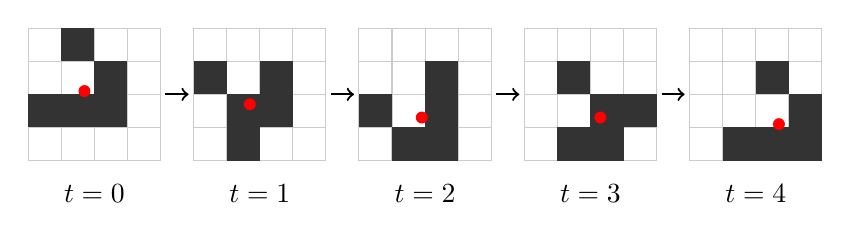
\begin{tikzpicture}[scale=0.42]
\draw[step=1,gray!40,thin] (0.0,-4) grid (4.0,0);
\fill[black!80] (0.0,-2) rectangle (1.0,-3);
\fill[black!80] (1.0,0) rectangle (2.0,-1);
\fill[black!80] (1.0,-2) rectangle (2.0,-3);
\fill[black!80] (2.0,-1) rectangle (3.0,-2);
\fill[black!80] (2.0,-2) rectangle (3.0,-3);
\fill[red] (1.7,-1.9) circle (0.18);
\node at (2.0,-5) {$t=0$};
\draw[->,thick] (4.15,-2) -- (4.85,-2);
\draw[step=1,gray!40,thin] (5.0,-4) grid (9.0,0);
\fill[black!80] (5.0,-1) rectangle (6.0,-2);
\fill[black!80] (6.0,-2) rectangle (7.0,-3);
\fill[black!80] (6.0,-3) rectangle (7.0,-4);
\fill[black!80] (7.0,-1) rectangle (8.0,-2);
\fill[black!80] (7.0,-2) rectangle (8.0,-3);
\fill[red] (6.7,-2.3) circle (0.18);
\node at (7.0,-5) {$t=1$};
\draw[->,thick] (9.15,-2) -- (9.85,-2);
\draw[step=1,gray!40,thin] (10.0,-4) grid (14.0,0);
\fill[black!80] (10.0,-2) rectangle (11.0,-3);
\fill[black!80] (11.0,-3) rectangle (12.0,-4);
\fill[black!80] (12.0,-1) rectangle (13.0,-2);
\fill[black!80] (12.0,-2) rectangle (13.0,-3);
\fill[black!80] (12.0,-3) rectangle (13.0,-4);
\fill[red] (11.9,-2.7) circle (0.18);
\node at (12.0,-5) {$t=2$};
\draw[->,thick] (14.15,-2) -- (14.85,-2);
\draw[step=1,gray!40,thin] (15.0,-4) grid (19.0,0);
\fill[black!80] (16.0,-1) rectangle (17.0,-2);
\fill[black!80] (16.0,-3) rectangle (17.0,-4);
\fill[black!80] (17.0,-2) rectangle (18.0,-3);
\fill[black!80] (17.0,-3) rectangle (18.0,-4);
\fill[black!80] (18.0,-2) rectangle (19.0,-3);
\fill[red] (17.3,-2.7) circle (0.18);
\node at (17.0,-5) {$t=3$};
\draw[->,thick] (19.15,-2) -- (19.85,-2);
\draw[step=1,gray!40,thin] (20.0,-4) grid (24.0,0);
\fill[black!80] (21.0,-3) rectangle (22.0,-4);
\fill[black!80] (22.0,-1) rectangle (23.0,-2);
\fill[black!80] (22.0,-3) rectangle (23.0,-4);
\fill[black!80] (23.0,-2) rectangle (24.0,-3);
\fill[black!80] (23.0,-3) rectangle (24.0,-4);
\fill[red] (22.7,-2.9) circle (0.18);
\node at (22.0,-5) {$t=4$};
\end{tikzpicture}
\caption{The Game of Life glider over one period ($B3/S23$), with $t=0$ live cells $\{(1,0),(2,1),(0,2),(1,2),(2,2)\}$. Black squares are live cells; the red dot is the centroid $\mathbf x_g$, the coarse-grained position. The configuration at $t=4$ is that at $t=0$ translated by $(1,1)$, and the centroid drifts from $(1.2,1.4)$ to $(2.2,2.4)$: the coarse object-dynamics $\Phi^{+}$ advances $\mathbf x_g$ by $(1,1)$ per object tick ($\lambda=4$ fine steps), exactly intertwining with the fine update, so the temporal-emergence defect vanishes for a lone glider.}
\label{fig::glider}
\end{figure}

\paragraph{Structural emergence: yes.} Since $\supp_{\Theta_\gamma}(\mathbf x_g)=L$ meets $|L|\geq2$ distinct cell-parts, clause~(2) of Definition~\ref{def::emerg} holds: the glider is structurally emergent over its cells. By Proposition~\ref{prop::recover} this is not a bookkeeping artefact---it depends on the average being a genuine non-projection transport. Here the valuations do real work: the emergent datum is the glider's \emph{velocity}, a non-additive function of the cells' liveness across two phases, not any single cell's state.

\paragraph{Temporal emergence: no, for a lone glider.} Let $\blacktriangle^t$ be the step to the object scale and $\Phi^{+}$ the coarse dynamics advancing one object tick by $\mathbf x_g\mapsto\mathbf x_g+(1,1)$, $\varphi_g\mapsto\varphi_g+1$, with rescaling $\lambda(1)=4$, i.e.\ $\zeta=\ln 4$ (one object tick subsumes four fine steps; the discrete case of Proposition~\ref{prop::resc}). For an isolated glider,
\[
\blacktriangle^t\!\left(\Phi_4(\beta_G)\right)=(\mathbf x_g+(1,1),\ \varphi_g)=\Phi^{+}\!\left(\blacktriangle^t(\beta_G)\right),
\]
so $\Delta^t_4=\varnothing$ and $\delta^t_4=0$: the coarse object-dynamics reproduces the coarse-grained fine dynamics exactly. A lone glider is therefore structurally but \emph{not} temporally emergent---the two notions genuinely come apart.

\paragraph{Temporal emergence: yes, at a collision.} Now take two gliders on a colliding course. The fine state $\beta$ has two disjoint object-supports $L_1,L_2$, and we coarse-grain to a two-object system $\mathcal S^{+}_2$ with elements $\{g_1,g_2\}$, absorption $a(\{c\})=g_j$ for $c\in L_j$ (undefined elsewhere), and the centroid/phase/velocity transport of the lone-glider case applied to each $L_j$. The coarse dynamics $\Phi^{+}$ advances the two objects independently, $\mathbf x_{g_j}\mapsto\mathbf x_{g_j}+(1,1)$, so $\Phi^{+}_{\lambda(t)\tau}(\blacktriangle^t(\beta))$ is the configuration in which both gliders have simply translated. The fine dynamics instead applies $B3/S23$ throughout: at contact the gliders react---mutual annihilation, a still life, or a new spaceship---so $\blacktriangle^t(\Phi_\tau(\beta))$ records a different multiset of objects.

To compare descriptions of different object-counts, fix once and for all---independently of $\beta$ and $\tau$---the catalogue $\mathcal O$ of all finite Life patterns up to translation, and let the shared host $\mathcal S^{+}_{\ast}$ have level set the finite subsets of $\mathcal O\times\mathbb Z^2$, a \emph{placed object} being a pattern-class together with an anchor, with the discrete pseudometric $d(A,B)=|A\,\triangle\,B|$. The coarse-graining is the clustering rule sending a fine state to the set of its maximal connected live components, each recorded as a placed object; it is defined for every $\beta$ and $\tau$ and lands in $\mathcal O\times\mathbb Z^2$ by construction, since every finite component is some pattern-class, so reaction products are catalogued rather than exceptional (annihilation being the empty set). Then
\[
\delta^t_\tau(\beta)=\bigl|\,\blacktriangle^t(\Phi_\tau(\beta))\ \triangle\ \Phi^{+}_{\lambda(t)\tau}(\blacktriangle^t(\beta))\,\bigr|>0,
\]
since the reacted configuration and the two-translated-gliders prediction differ on at least one object. The collision is therefore both structurally and temporally emergent, whereas the lone glider was structurally emergent only. This is exactly the discrimination the framework is meant to deliver: emergence is localised at the coarse-graining, and the two cases receive different verdicts on the temporal axis while both pass the structural one.

\section{Conclusion}

The definitions are abstract, but their intended use is concrete. In a gas, molecules form the lower-level elements; regions carrying pressure and temperature form a coarser system. Structural transport records the passage from molecular velocities and collisions to thermodynamic quantities. The coarse description is reductive where it only discards detail, but emergent when it introduces relations or contextual variables not present in the non-interacting aggregate of regions. The same example also shows why reduction and emergence should not be treated as mutually exclusive slogans: temperature may be reducible as an aggregate variable and still participate in laws that are not conveniently stated at the molecular level.

In a cellular organism, cells can be holons: each has internal organization, and each is a part of tissue-level organization. The tissue is not merely the disjoint union of cells, since extracellular context, signalling and mechanical coupling enter the coarse description. An organ is again a whole relative to tissues and a part relative to an organism. This is the ordinary biological reason for the holarchic vocabulary: it is very rarely useful to say that only one of these levels is real. What matters is how they constrain, summarize and produce each other.

In artificial life, candidate holons would be coherent aggregates: gliders, particle-life clusters, Lenia life-forms, or other persistent patterns. Structural emergence would be read from the transport producing their coarse relations; temporal emergence from the defect comparing microscopic evolution with aggregate evolution. Such systems are especially useful because the microscopic rules are known. If emergence is found there, it is not because the underlying rules are mysterious, but because the relevant whole is obtained only after a non-trivial passage of description.

The next step is self-similarity. The present paper gives the domain on which a similarity measure should act: systems, structural transports, coarse-grainings and dynamics. A self-similar holarchy should preserve enough relational and dynamical form across scale to deserve the name, but different applications may compare different data: relations, valuations, supports, temporal defects, distributions of structures, or invariants derived from network theory, persistent homology or information theory. The important point is that similarity should compare not only systems at isolated levels, but also the transports between them.

Two generalizations are immediate. First, one may relax adjacency and allow interlevel interactions not mediated by a single coarse-graining flow, including holons assembled from parts living at different levels. Second, one may study centralization internal to holarchies: an emergent supersystem may coordinate or constrain its parts without being an external controller. In that sense, a complex system can be decentralized from the perspective of its atoms and still contain centralizing units at higher emergent levels. This is precisely why holarchies seem useful: they keep parts, wholes, boundaries and scales in one formal picture.

We close by emphasizing the modesty of the proposal. The definitions above do not solve the problem of emergence, nor do they decide which systems are important. They provide a language in which these questions can be posed with fewer hidden assumptions. In particular, they separate the existence of parts, the existence of levels, the act of coarse-graining, the presence of structural emergence and the presence of temporal emergence. This separation is, we believe, the minimum needed before one can study the more demanding question that motivated the work: whether some complex systems are not only holarchic, but self-similar across their holarchic structure.

This also suggests a practical research programme. One may start with an artificial-life model whose microscopic rule is known, choose candidate aggregates by clustering or persistence, construct structural transports for the variables used to describe them, and then measure the temporal defect across scales. If the same kind of transport reappears at several levels, one has a concrete candidate for self-similarity. If it does not, the framework still says where the analogy failed: in the decomposition, in the transport, in the dynamics, or in the comparison between scales.

The usefulness of the framework will therefore depend less on the elegance of the definitions than on whether they make these failures legible. If a proposed holon cannot be enclosed by a higher-level system, the problem is mereological. If a coarse variable cannot be transported from lower-level data except by an arbitrary constant, the problem is structural. If the coarse dynamics fails to match any rescaled microscopic evolution, the problem is temporal. These are different failures, and a theory of complex systems should not confuse them. The present formalism is an attempt to keep them separated while still allowing them to appear in the same object.

% ---- Bibliography ----
\bibliographystyle{splncs04}
\bibliography{mybib}

\end{document}
